\documentclass[twoside]{book}

% Packages required by doxygen
\usepackage{fixltx2e}
\usepackage{calc}
\usepackage{doxygen}
\usepackage{graphicx}
\usepackage[utf8]{inputenc}
\usepackage{makeidx}
\usepackage{multicol}
\usepackage{multirow}
\PassOptionsToPackage{warn}{textcomp}
\usepackage{textcomp}
\usepackage[nointegrals]{wasysym}
\usepackage[table]{xcolor}

% Font selection
\usepackage[T1]{fontenc}
\usepackage{mathptmx}
\usepackage[scaled=.90]{helvet}
\usepackage{courier}
\usepackage{amssymb}
\usepackage{sectsty}
\renewcommand{\familydefault}{\sfdefault}
\allsectionsfont{%
  \fontseries{bc}\selectfont%
  \color{darkgray}%
}
\renewcommand{\DoxyLabelFont}{%
  \fontseries{bc}\selectfont%
  \color{darkgray}%
}
\newcommand{\+}{\discretionary{\mbox{\scriptsize$\hookleftarrow$}}{}{}}

% Page & text layout
\usepackage{geometry}
\geometry{%
  a4paper,%
  top=2.5cm,%
  bottom=2.5cm,%
  left=2.5cm,%
  right=2.5cm%
}
\tolerance=750
\hfuzz=15pt
\hbadness=750
\setlength{\emergencystretch}{15pt}
\setlength{\parindent}{0cm}
\setlength{\parskip}{0.2cm}
\makeatletter
\renewcommand{\paragraph}{%
  \@startsection{paragraph}{4}{0ex}{-1.0ex}{1.0ex}{%
    \normalfont\normalsize\bfseries\SS@parafont%
  }%
}
\renewcommand{\subparagraph}{%
  \@startsection{subparagraph}{5}{0ex}{-1.0ex}{1.0ex}{%
    \normalfont\normalsize\bfseries\SS@subparafont%
  }%
}
\makeatother

% Headers & footers
\usepackage{fancyhdr}
\pagestyle{fancyplain}
\fancyhead[LE]{\fancyplain{}{\bfseries\thepage}}
\fancyhead[CE]{\fancyplain{}{}}
\fancyhead[RE]{\fancyplain{}{\bfseries\leftmark}}
\fancyhead[LO]{\fancyplain{}{\bfseries\rightmark}}
\fancyhead[CO]{\fancyplain{}{}}
\fancyhead[RO]{\fancyplain{}{\bfseries\thepage}}
\fancyfoot[LE]{\fancyplain{}{}}
\fancyfoot[CE]{\fancyplain{}{}}
\fancyfoot[RE]{\fancyplain{}{\bfseries\scriptsize Generated on Tue May 3 2016 20\+:56\+:18 for sdem\+App by Doxygen }}
\fancyfoot[LO]{\fancyplain{}{\bfseries\scriptsize Generated on Tue May 3 2016 20\+:56\+:18 for sdem\+App by Doxygen }}
\fancyfoot[CO]{\fancyplain{}{}}
\fancyfoot[RO]{\fancyplain{}{}}
\renewcommand{\footrulewidth}{0.4pt}
\renewcommand{\chaptermark}[1]{%
  \markboth{#1}{}%
}
\renewcommand{\sectionmark}[1]{%
  \markright{\thesection\ #1}%
}

% Indices & bibliography
\usepackage{natbib}
\usepackage[titles]{tocloft}
\setcounter{tocdepth}{3}
\setcounter{secnumdepth}{5}
\makeindex

% Hyperlinks (required, but should be loaded last)
\usepackage{ifpdf}
\ifpdf
  \usepackage[pdftex,pagebackref=true]{hyperref}
\else
  \usepackage[ps2pdf,pagebackref=true]{hyperref}
\fi
\hypersetup{%
  colorlinks=true,%
  linkcolor=blue,%
  citecolor=blue,%
  unicode%
}

% Custom commands
\newcommand{\clearemptydoublepage}{%
  \newpage{\pagestyle{empty}\cleardoublepage}%
}


%===== C O N T E N T S =====

\begin{document}

% Titlepage & ToC
\hypersetup{pageanchor=false,
             bookmarks=true,
             bookmarksnumbered=true,
             pdfencoding=unicode
            }
\pagenumbering{roman}
\begin{titlepage}
\vspace*{7cm}
\begin{center}%
{\Large sdem\+App }\\
\vspace*{1cm}
{\large Generated by Doxygen 1.8.8}\\
\vspace*{0.5cm}
{\small Tue May 3 2016 20:56:18}\\
\end{center}
\end{titlepage}
\clearemptydoublepage
\tableofcontents
\clearemptydoublepage
\pagenumbering{arabic}
\hypersetup{pageanchor=true}

%--- Begin generated contents ---
\chapter{Namespace Index}
\section{Namespace List}
Here is a list of all namespaces with brief descriptions\+:\begin{DoxyCompactList}
\item\contentsline{section}{\hyperlink{namespacesdem}{sdem} }{\pageref{namespacesdem}}{}
\item\contentsline{section}{\hyperlink{namespacesdem_1_1unimore}{sdem.\+unimore} }{\pageref{namespacesdem_1_1unimore}}{}
\item\contentsline{section}{\hyperlink{namespacesdem_1_1unimore_1_1com}{sdem.\+unimore.\+com} }{\pageref{namespacesdem_1_1unimore_1_1com}}{}
\item\contentsline{section}{\hyperlink{namespacesdem_1_1unimore_1_1com_1_1sdemapp}{sdem.\+unimore.\+com.\+sdemapp} }{\pageref{namespacesdem_1_1unimore_1_1com_1_1sdemapp}}{}
\end{DoxyCompactList}

\chapter{Hierarchical Index}
\section{Class Hierarchy}
This inheritance list is sorted roughly, but not completely, alphabetically\+:\begin{DoxyCompactList}
\item Callback\begin{DoxyCompactList}
\item \contentsline{section}{sdem.\+unimore.\+com.\+sdemapp.\+Draw\+View}{\pageref{classsdem_1_1unimore_1_1com_1_1sdemapp_1_1_draw_view}}{}
\end{DoxyCompactList}
\item \contentsline{section}{detection\+\_\+marker}{\pageref{classdetection__marker}}{}
\item App\+Compat\+Activity\begin{DoxyCompactList}
\item \contentsline{section}{sdem.\+unimore.\+com.\+sdemapp.\+Fullscreen\+Activity}{\pageref{classsdem_1_1unimore_1_1com_1_1sdemapp_1_1_fullscreen_activity}}{}
\end{DoxyCompactList}
\item Surface\+View\begin{DoxyCompactList}
\item \contentsline{section}{sdem.\+unimore.\+com.\+sdemapp.\+Draw\+View}{\pageref{classsdem_1_1unimore_1_1com_1_1sdemapp_1_1_draw_view}}{}
\end{DoxyCompactList}
\end{DoxyCompactList}

\chapter{Class Index}
\section{Class List}
Here are the classes, structs, unions and interfaces with brief descriptions\+:\begin{DoxyCompactList}
\item\contentsline{section}{\hyperlink{classdetection__marker}{detection\+\_\+marker} }{\pageref{classdetection__marker}}{}
\item\contentsline{section}{\hyperlink{classsdem_1_1unimore_1_1com_1_1sdemapp_1_1_draw_view}{sdem.\+unimore.\+com.\+sdemapp.\+Draw\+View} }{\pageref{classsdem_1_1unimore_1_1com_1_1sdemapp_1_1_draw_view}}{}
\item\contentsline{section}{\hyperlink{classsdem_1_1unimore_1_1com_1_1sdemapp_1_1_fullscreen_activity}{sdem.\+unimore.\+com.\+sdemapp.\+Fullscreen\+Activity} }{\pageref{classsdem_1_1unimore_1_1com_1_1sdemapp_1_1_fullscreen_activity}}{}
\end{DoxyCompactList}

\chapter{File Index}
\section{File List}
Here is a list of all files with brief descriptions\+:\begin{DoxyCompactList}
\item\contentsline{section}{/home/francesco/\+Android\+Studio\+Projects/sdem\+\_\+app/app/src/main/java/\hyperlink{intro__app_8cpp}{intro\+\_\+app.\+cpp} }{\pageref{intro__app_8cpp}}{}
\item\contentsline{section}{/home/francesco/\+Android\+Studio\+Projects/sdem\+\_\+app/app/src/main/java/sdem/unimore/com/sdemapp/\hyperlink{_camera_view_8java}{Camera\+View.\+java} }{\pageref{_camera_view_8java}}{}
\item\contentsline{section}{/home/francesco/\+Android\+Studio\+Projects/sdem\+\_\+app/app/src/main/java/sdem/unimore/com/sdemapp/\hyperlink{_draw_view_8java}{Draw\+View.\+java} }{\pageref{_draw_view_8java}}{}
\item\contentsline{section}{/home/francesco/\+Android\+Studio\+Projects/sdem\+\_\+app/app/src/main/java/sdem/unimore/com/sdemapp/\hyperlink{_fullscreen_activity_8java}{Fullscreen\+Activity.\+java} }{\pageref{_fullscreen_activity_8java}}{}
\item\contentsline{section}{/home/francesco/\+Android\+Studio\+Projects/sdem\+\_\+app/app/src/main/jni/\hyperlink{detection_8cpp}{detection.\+cpp} }{\pageref{detection_8cpp}}{}
\item\contentsline{section}{/home/francesco/\+Android\+Studio\+Projects/sdem\+\_\+app/app/src/main/jni/\hyperlink{detection_8h}{detection.\+h} }{\pageref{detection_8h}}{}
\item\contentsline{section}{/home/francesco/\+Android\+Studio\+Projects/sdem\+\_\+app/app/src/main/jni/\hyperlink{_sdem_app_j_n_i_8cpp}{Sdem\+App\+J\+N\+I.\+cpp} }{\pageref{_sdem_app_j_n_i_8cpp}}{}
\end{DoxyCompactList}

\chapter{Namespace Documentation}
\hypertarget{namespacesdem}{\section{Package sdem}
\label{namespacesdem}\index{sdem@{sdem}}
}
\subsection*{Packages}
\begin{DoxyCompactItemize}
\item 
package \hyperlink{namespacesdem_1_1unimore}{unimore}
\end{DoxyCompactItemize}

\hypertarget{namespacesdem_1_1unimore}{\section{Package sdem.\+unimore}
\label{namespacesdem_1_1unimore}\index{sdem.\+unimore@{sdem.\+unimore}}
}
\subsection*{Packages}
\begin{DoxyCompactItemize}
\item 
package \hyperlink{namespacesdem_1_1unimore_1_1com}{com}
\end{DoxyCompactItemize}

\hypertarget{namespacesdem_1_1unimore_1_1com}{\section{Package sdem.\+unimore.\+com}
\label{namespacesdem_1_1unimore_1_1com}\index{sdem.\+unimore.\+com@{sdem.\+unimore.\+com}}
}
\subsection*{Packages}
\begin{DoxyCompactItemize}
\item 
package \hyperlink{namespacesdem_1_1unimore_1_1com_1_1sdemapp}{sdemapp}
\end{DoxyCompactItemize}

\hypertarget{namespacesdem_1_1unimore_1_1com_1_1sdemapp}{\section{Package sdem.\+unimore.\+com.\+sdemapp}
\label{namespacesdem_1_1unimore_1_1com_1_1sdemapp}\index{sdem.\+unimore.\+com.\+sdemapp@{sdem.\+unimore.\+com.\+sdemapp}}
}
\subsection*{Classes}
\begin{DoxyCompactItemize}
\item 
class \hyperlink{classsdem_1_1unimore_1_1com_1_1sdemapp_1_1_draw_view}{Draw\+View}
\item 
class \hyperlink{classsdem_1_1unimore_1_1com_1_1sdemapp_1_1_fullscreen_activity}{Fullscreen\+Activity}
\end{DoxyCompactItemize}

\chapter{Class Documentation}
\hypertarget{classdetection__marker}{\section{detection\+\_\+marker Class Reference}
\label{classdetection__marker}\index{detection\+\_\+marker@{detection\+\_\+marker}}
}


{\ttfamily \#include $<$detection.\+h$>$}

\subsection*{Public Member Functions}
\begin{DoxyCompactItemize}
\item 
\hyperlink{classdetection__marker_a78703d9cfece4550684a3f6e0dfd659b}{detection\+\_\+marker} (P\+R\+E\+D\+E\+F\+I\+N\+E\+D\+\_\+\+D\+I\+C\+T\+I\+O\+N\+A\+R\+Y\+\_\+\+N\+A\+M\+E name)
\item 
const vector$<$ int $>$ \& \hyperlink{classdetection__marker_a486d89e7f7008d87a1c3c26c89ad3b74}{ids} () const 
\item 
const vector$<$ vector$<$ Point2f $>$ $>$ \& \hyperlink{classdetection__marker_a243c4a54a4b9d9c084672660e5d47f39}{corners} () const 
\item 
const Mat \& \hyperlink{classdetection__marker_a770b0b3075bf960621006f7f939b9757}{img} () const 
\item 
void \hyperlink{classdetection__marker_a08cd89907df009bce97bb5a6561074e6}{detect\+And\+Draw} (Mat \&in\+Image)
\item 
void \hyperlink{classdetection__marker_a4149fb9467f5cc15b1086c548821d925}{detect} (Mat \&in\+Image)
\end{DoxyCompactItemize}


\subsection{Detailed Description}
Classe di gestione dei marker aruco. 

Definition at line 22 of file detection.\+h.



\subsection{Constructor \& Destructor Documentation}
\hypertarget{classdetection__marker_a78703d9cfece4550684a3f6e0dfd659b}{\index{detection\+\_\+marker@{detection\+\_\+marker}!detection\+\_\+marker@{detection\+\_\+marker}}
\index{detection\+\_\+marker@{detection\+\_\+marker}!detection\+\_\+marker@{detection\+\_\+marker}}
\subsubsection[{detection\+\_\+marker}]{\setlength{\rightskip}{0pt plus 5cm}detection\+\_\+marker\+::detection\+\_\+marker (
\begin{DoxyParamCaption}
\item[{P\+R\+E\+D\+E\+F\+I\+N\+E\+D\+\_\+\+D\+I\+C\+T\+I\+O\+N\+A\+R\+Y\+\_\+\+N\+A\+M\+E}]{name}
\end{DoxyParamCaption}
)}}\label{classdetection__marker_a78703d9cfece4550684a3f6e0dfd659b}
Costruttore dell'oggetto detection marker. Prende come parametro il nome del dizionario dei marker aruco che si vogliono visualizzare.


\begin{DoxyParams}{Parameters}
{\em name} & nome del dizionario aruco. \\
\hline
\end{DoxyParams}


Definition at line 15 of file detection.\+cpp.



\subsection{Member Function Documentation}
\hypertarget{classdetection__marker_a243c4a54a4b9d9c084672660e5d47f39}{\index{detection\+\_\+marker@{detection\+\_\+marker}!corners@{corners}}
\index{corners@{corners}!detection\+\_\+marker@{detection\+\_\+marker}}
\subsubsection[{corners}]{\setlength{\rightskip}{0pt plus 5cm}const vector$<$ vector$<$ Point2f $>$ $>$ \& detection\+\_\+marker\+::corners (
\begin{DoxyParamCaption}
{}
\end{DoxyParamCaption}
) const}}\label{classdetection__marker_a243c4a54a4b9d9c084672660e5d47f39}
Restituisce le coordinate dei vertici dei marker che sono stati riconosciuti, nell'ultima chiamata, da uno dei metodi detect\+And\+Draw o detect.

\begin{DoxyReturn}{Returns}
reference a vettore di Point2f contenente i punti che rappresentano la posizione a schermo dei vertici dei marker riconosciuti. 
\end{DoxyReturn}


Definition at line 18 of file detection.\+cpp.

\hypertarget{classdetection__marker_a4149fb9467f5cc15b1086c548821d925}{\index{detection\+\_\+marker@{detection\+\_\+marker}!detect@{detect}}
\index{detect@{detect}!detection\+\_\+marker@{detection\+\_\+marker}}
\subsubsection[{detect}]{\setlength{\rightskip}{0pt plus 5cm}void detection\+\_\+marker\+::detect (
\begin{DoxyParamCaption}
\item[{Mat \&}]{in\+Image}
\end{DoxyParamCaption}
)}}\label{classdetection__marker_a4149fb9467f5cc15b1086c548821d925}
Esegue la procedura di detection su in\+Image.


\begin{DoxyParams}{Parameters}
{\em in\+Image} & oggetto Mat che rappresenta il frame su cui eseguire la detection. \\
\hline
\end{DoxyParams}


Definition at line 28 of file detection.\+cpp.

\hypertarget{classdetection__marker_a08cd89907df009bce97bb5a6561074e6}{\index{detection\+\_\+marker@{detection\+\_\+marker}!detect\+And\+Draw@{detect\+And\+Draw}}
\index{detect\+And\+Draw@{detect\+And\+Draw}!detection\+\_\+marker@{detection\+\_\+marker}}
\subsubsection[{detect\+And\+Draw}]{\setlength{\rightskip}{0pt plus 5cm}void detection\+\_\+marker\+::detect\+And\+Draw (
\begin{DoxyParamCaption}
\item[{Mat \&}]{in\+Image}
\end{DoxyParamCaption}
)}}\label{classdetection__marker_a08cd89907df009bce97bb5a6561074e6}
Esegue la procedura di detection su in\+Image. Disegna direttamente sul frame il contorno dei marker individuati correttamente.


\begin{DoxyParams}{Parameters}
{\em in\+Image} & oggetto Mat che rappresenta il frame su cui eseguire la detection. \\
\hline
\end{DoxyParams}


Definition at line 21 of file detection.\+cpp.

\hypertarget{classdetection__marker_a486d89e7f7008d87a1c3c26c89ad3b74}{\index{detection\+\_\+marker@{detection\+\_\+marker}!ids@{ids}}
\index{ids@{ids}!detection\+\_\+marker@{detection\+\_\+marker}}
\subsubsection[{ids}]{\setlength{\rightskip}{0pt plus 5cm}const vector$<$ int $>$ \& detection\+\_\+marker\+::ids (
\begin{DoxyParamCaption}
{}
\end{DoxyParamCaption}
) const}}\label{classdetection__marker_a486d89e7f7008d87a1c3c26c89ad3b74}
Restituisce gli identificatori dei marker che sono stati riconosciuti, nell'ultima chiamata, da uno dei metodi detect\+And\+Draw o detect.

\begin{DoxyReturn}{Returns}
reference a vettore di interi contenente gli identificatori dei marker riconosciuti. 
\end{DoxyReturn}


Definition at line 17 of file detection.\+cpp.

\hypertarget{classdetection__marker_a770b0b3075bf960621006f7f939b9757}{\index{detection\+\_\+marker@{detection\+\_\+marker}!img@{img}}
\index{img@{img}!detection\+\_\+marker@{detection\+\_\+marker}}
\subsubsection[{img}]{\setlength{\rightskip}{0pt plus 5cm}const Mat \& detection\+\_\+marker\+::img (
\begin{DoxyParamCaption}
{}
\end{DoxyParamCaption}
) const}}\label{classdetection__marker_a770b0b3075bf960621006f7f939b9757}
Restituisce l'oggetto Mat corrispondente al frame corrente su cui è stato invocato uno dei metodi detect\+And\+Draw o detect.

\begin{DoxyReturn}{Returns}
reference a Mat. 
\end{DoxyReturn}


Definition at line 19 of file detection.\+cpp.



The documentation for this class was generated from the following files\+:\begin{DoxyCompactItemize}
\item 
/home/francesco/\+Android\+Studio\+Projects/sdem\+\_\+app/app/src/main/jni/\hyperlink{detection_8h}{detection.\+h}\item 
/home/francesco/\+Android\+Studio\+Projects/sdem\+\_\+app/app/src/main/jni/\hyperlink{detection_8cpp}{detection.\+cpp}\end{DoxyCompactItemize}

\hypertarget{classsdem_1_1unimore_1_1com_1_1sdemapp_1_1_draw_view}{\section{sdem.\+unimore.\+com.\+sdemapp.\+Draw\+View Class Reference}
\label{classsdem_1_1unimore_1_1com_1_1sdemapp_1_1_draw_view}\index{sdem.\+unimore.\+com.\+sdemapp.\+Draw\+View@{sdem.\+unimore.\+com.\+sdemapp.\+Draw\+View}}
}
Inheritance diagram for sdem.\+unimore.\+com.\+sdemapp.\+Draw\+View\+:\begin{figure}[H]
\begin{center}
\leavevmode
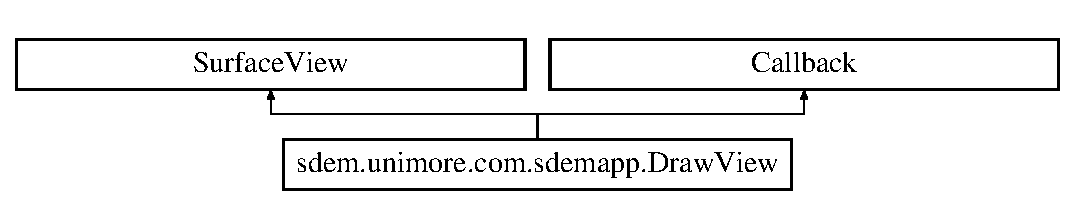
\includegraphics[height=2.000000cm]{classsdem_1_1unimore_1_1com_1_1sdemapp_1_1_draw_view}
\end{center}
\end{figure}
\subsection*{Public Member Functions}
\begin{DoxyCompactItemize}
\item 
\hyperlink{classsdem_1_1unimore_1_1com_1_1sdemapp_1_1_draw_view_a0f33e842727aa93495a965aa58757cf6}{Draw\+View} (Context context, Attribute\+Set attrs)
\item 
void \hyperlink{classsdem_1_1unimore_1_1com_1_1sdemapp_1_1_draw_view_aae745ca136fcbfcac69ebdaa4d106711}{draw\+Corners} (float\mbox{[}$\,$\mbox{]} corners, int\mbox{[}$\,$\mbox{]} id\+List)
\item 
void \hyperlink{classsdem_1_1unimore_1_1com_1_1sdemapp_1_1_draw_view_a5a538e420c4205dc2db79429f9de17f0}{draw\+Text\+Centred} (Canvas canvas, Paint paint, String text, float cx, float cy)
\item 
void \hyperlink{classsdem_1_1unimore_1_1com_1_1sdemapp_1_1_draw_view_adac404d58277c2e02759e52a007ff2f2}{surface\+Created} (Surface\+Holder holder)
\item 
void \hyperlink{classsdem_1_1unimore_1_1com_1_1sdemapp_1_1_draw_view_ac654c04ec20230794d1f7d4205ff6ccc}{surface\+Changed} (Surface\+Holder holder, int format, int width, int height)
\item 
void \hyperlink{classsdem_1_1unimore_1_1com_1_1sdemapp_1_1_draw_view_ada0d09df8995e1a3b2356d3d99d79808}{surface\+Destroyed} (Surface\+Holder holder)
\end{DoxyCompactItemize}


\subsection{Detailed Description}
Classe di gestione delle immagini disegnate sopra alla preview dei frame. 

Definition at line 23 of file Draw\+View.\+java.



\subsection{Constructor \& Destructor Documentation}
\hypertarget{classsdem_1_1unimore_1_1com_1_1sdemapp_1_1_draw_view_a0f33e842727aa93495a965aa58757cf6}{\index{sdem\+::unimore\+::com\+::sdemapp\+::\+Draw\+View@{sdem\+::unimore\+::com\+::sdemapp\+::\+Draw\+View}!Draw\+View@{Draw\+View}}
\index{Draw\+View@{Draw\+View}!sdem\+::unimore\+::com\+::sdemapp\+::\+Draw\+View@{sdem\+::unimore\+::com\+::sdemapp\+::\+Draw\+View}}
\subsubsection[{Draw\+View}]{\setlength{\rightskip}{0pt plus 5cm}sdem.\+unimore.\+com.\+sdemapp.\+Draw\+View.\+Draw\+View (
\begin{DoxyParamCaption}
\item[{Context}]{context, }
\item[{Attribute\+Set}]{attrs}
\end{DoxyParamCaption}
)\hspace{0.3cm}{\ttfamily [inline]}}}\label{classsdem_1_1unimore_1_1com_1_1sdemapp_1_1_draw_view_a0f33e842727aa93495a965aa58757cf6}
Costruttore oggetto Drawview. Al suo interno vengono impostati i valori di line\+Paint e text\+Paint oltre che gli attributi necessari ad avere una superficie trasparente.


\begin{DoxyParams}{Parameters}
{\em context} & context \\
\hline
{\em attrs} & attrs \\
\hline
\end{DoxyParams}


Definition at line 36 of file Draw\+View.\+java.



\subsection{Member Function Documentation}
\hypertarget{classsdem_1_1unimore_1_1com_1_1sdemapp_1_1_draw_view_aae745ca136fcbfcac69ebdaa4d106711}{\index{sdem\+::unimore\+::com\+::sdemapp\+::\+Draw\+View@{sdem\+::unimore\+::com\+::sdemapp\+::\+Draw\+View}!draw\+Corners@{draw\+Corners}}
\index{draw\+Corners@{draw\+Corners}!sdem\+::unimore\+::com\+::sdemapp\+::\+Draw\+View@{sdem\+::unimore\+::com\+::sdemapp\+::\+Draw\+View}}
\subsubsection[{draw\+Corners}]{\setlength{\rightskip}{0pt plus 5cm}void sdem.\+unimore.\+com.\+sdemapp.\+Draw\+View.\+draw\+Corners (
\begin{DoxyParamCaption}
\item[{float\mbox{[}$\,$\mbox{]}}]{corners, }
\item[{int\mbox{[}$\,$\mbox{]}}]{id\+List}
\end{DoxyParamCaption}
)\hspace{0.3cm}{\ttfamily [inline]}}}\label{classsdem_1_1unimore_1_1com_1_1sdemapp_1_1_draw_view_aae745ca136fcbfcac69ebdaa4d106711}
Metodo di disegno del contorno di un marker. Prende in ingresso la lista di angoli in formato float e genera un poligono di 4 lati ogni 4 coppie (x,y).


\begin{DoxyParams}{Parameters}
{\em corners} & vettore angoli \\
\hline
{\em id\+List} & vettore I\+Ds \\
\hline
\end{DoxyParams}


Definition at line 75 of file Draw\+View.\+java.

\hypertarget{classsdem_1_1unimore_1_1com_1_1sdemapp_1_1_draw_view_a5a538e420c4205dc2db79429f9de17f0}{\index{sdem\+::unimore\+::com\+::sdemapp\+::\+Draw\+View@{sdem\+::unimore\+::com\+::sdemapp\+::\+Draw\+View}!draw\+Text\+Centred@{draw\+Text\+Centred}}
\index{draw\+Text\+Centred@{draw\+Text\+Centred}!sdem\+::unimore\+::com\+::sdemapp\+::\+Draw\+View@{sdem\+::unimore\+::com\+::sdemapp\+::\+Draw\+View}}
\subsubsection[{draw\+Text\+Centred}]{\setlength{\rightskip}{0pt plus 5cm}void sdem.\+unimore.\+com.\+sdemapp.\+Draw\+View.\+draw\+Text\+Centred (
\begin{DoxyParamCaption}
\item[{Canvas}]{canvas, }
\item[{Paint}]{paint, }
\item[{String}]{text, }
\item[{float}]{cx, }
\item[{float}]{cy}
\end{DoxyParamCaption}
)\hspace{0.3cm}{\ttfamily [inline]}}}\label{classsdem_1_1unimore_1_1com_1_1sdemapp_1_1_draw_view_a5a538e420c4205dc2db79429f9de17f0}


Definition at line 123 of file Draw\+View.\+java.

\hypertarget{classsdem_1_1unimore_1_1com_1_1sdemapp_1_1_draw_view_ac654c04ec20230794d1f7d4205ff6ccc}{\index{sdem\+::unimore\+::com\+::sdemapp\+::\+Draw\+View@{sdem\+::unimore\+::com\+::sdemapp\+::\+Draw\+View}!surface\+Changed@{surface\+Changed}}
\index{surface\+Changed@{surface\+Changed}!sdem\+::unimore\+::com\+::sdemapp\+::\+Draw\+View@{sdem\+::unimore\+::com\+::sdemapp\+::\+Draw\+View}}
\subsubsection[{surface\+Changed}]{\setlength{\rightskip}{0pt plus 5cm}void sdem.\+unimore.\+com.\+sdemapp.\+Draw\+View.\+surface\+Changed (
\begin{DoxyParamCaption}
\item[{Surface\+Holder}]{holder, }
\item[{int}]{format, }
\item[{int}]{width, }
\item[{int}]{height}
\end{DoxyParamCaption}
)\hspace{0.3cm}{\ttfamily [inline]}}}\label{classsdem_1_1unimore_1_1com_1_1sdemapp_1_1_draw_view_ac654c04ec20230794d1f7d4205ff6ccc}
Override Surface\+Holder.\+Callback


\begin{DoxyParams}{Parameters}
{\em holder} & holder \\
\hline
{\em format} & format \\
\hline
{\em width} & width \\
\hline
{\em height} & height \\
\hline
\end{DoxyParams}


Definition at line 147 of file Draw\+View.\+java.

\hypertarget{classsdem_1_1unimore_1_1com_1_1sdemapp_1_1_draw_view_adac404d58277c2e02759e52a007ff2f2}{\index{sdem\+::unimore\+::com\+::sdemapp\+::\+Draw\+View@{sdem\+::unimore\+::com\+::sdemapp\+::\+Draw\+View}!surface\+Created@{surface\+Created}}
\index{surface\+Created@{surface\+Created}!sdem\+::unimore\+::com\+::sdemapp\+::\+Draw\+View@{sdem\+::unimore\+::com\+::sdemapp\+::\+Draw\+View}}
\subsubsection[{surface\+Created}]{\setlength{\rightskip}{0pt plus 5cm}void sdem.\+unimore.\+com.\+sdemapp.\+Draw\+View.\+surface\+Created (
\begin{DoxyParamCaption}
\item[{Surface\+Holder}]{holder}
\end{DoxyParamCaption}
)\hspace{0.3cm}{\ttfamily [inline]}}}\label{classsdem_1_1unimore_1_1com_1_1sdemapp_1_1_draw_view_adac404d58277c2e02759e52a007ff2f2}
Override Surface\+Holder.\+Callback


\begin{DoxyParams}{Parameters}
{\em holder} & holder \\
\hline
\end{DoxyParams}


Definition at line 134 of file Draw\+View.\+java.

\hypertarget{classsdem_1_1unimore_1_1com_1_1sdemapp_1_1_draw_view_ada0d09df8995e1a3b2356d3d99d79808}{\index{sdem\+::unimore\+::com\+::sdemapp\+::\+Draw\+View@{sdem\+::unimore\+::com\+::sdemapp\+::\+Draw\+View}!surface\+Destroyed@{surface\+Destroyed}}
\index{surface\+Destroyed@{surface\+Destroyed}!sdem\+::unimore\+::com\+::sdemapp\+::\+Draw\+View@{sdem\+::unimore\+::com\+::sdemapp\+::\+Draw\+View}}
\subsubsection[{surface\+Destroyed}]{\setlength{\rightskip}{0pt plus 5cm}void sdem.\+unimore.\+com.\+sdemapp.\+Draw\+View.\+surface\+Destroyed (
\begin{DoxyParamCaption}
\item[{Surface\+Holder}]{holder}
\end{DoxyParamCaption}
)\hspace{0.3cm}{\ttfamily [inline]}}}\label{classsdem_1_1unimore_1_1com_1_1sdemapp_1_1_draw_view_ada0d09df8995e1a3b2356d3d99d79808}
Override Surface\+Holder.\+Callback


\begin{DoxyParams}{Parameters}
{\em holder} & holder \\
\hline
\end{DoxyParams}


Definition at line 157 of file Draw\+View.\+java.



The documentation for this class was generated from the following file\+:\begin{DoxyCompactItemize}
\item 
/home/francesco/\+Android\+Studio\+Projects/sdem\+\_\+app/app/src/main/java/sdem/unimore/com/sdemapp/\hyperlink{_draw_view_8java}{Draw\+View.\+java}\end{DoxyCompactItemize}

\hypertarget{classsdem_1_1unimore_1_1com_1_1sdemapp_1_1_fullscreen_activity}{\section{sdem.\+unimore.\+com.\+sdemapp.\+Fullscreen\+Activity Class Reference}
\label{classsdem_1_1unimore_1_1com_1_1sdemapp_1_1_fullscreen_activity}\index{sdem.\+unimore.\+com.\+sdemapp.\+Fullscreen\+Activity@{sdem.\+unimore.\+com.\+sdemapp.\+Fullscreen\+Activity}}
}
Inheritance diagram for sdem.\+unimore.\+com.\+sdemapp.\+Fullscreen\+Activity\+:\begin{figure}[H]
\begin{center}
\leavevmode
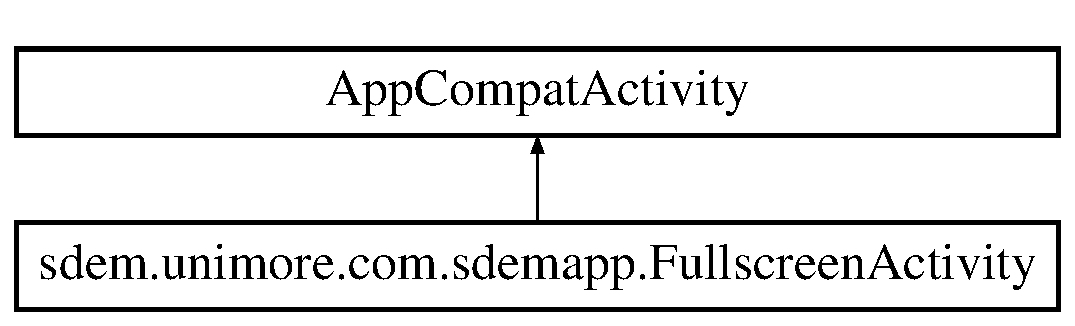
\includegraphics[height=2.000000cm]{classsdem_1_1unimore_1_1com_1_1sdemapp_1_1_fullscreen_activity}
\end{center}
\end{figure}
\subsection*{Public Member Functions}
\begin{DoxyCompactItemize}
\item 
void \hyperlink{classsdem_1_1unimore_1_1com_1_1sdemapp_1_1_fullscreen_activity_aa00cf64d5669932c3b4ca55e3dee382c}{on\+Request\+Permissions\+Result} (int request\+Code, String permissions\mbox{[}$\,$\mbox{]}, int\mbox{[}$\,$\mbox{]} grant\+Results)
\end{DoxyCompactItemize}
\subsection*{Protected Member Functions}
\begin{DoxyCompactItemize}
\item 
void \hyperlink{classsdem_1_1unimore_1_1com_1_1sdemapp_1_1_fullscreen_activity_aa47fc4234b35e26366da2aeded279ed4}{on\+Create} (Bundle saved\+Instance\+State)
\item 
void \hyperlink{classsdem_1_1unimore_1_1com_1_1sdemapp_1_1_fullscreen_activity_ab4610475ff6a0a0099971f041a95f5ba}{on\+Resume} ()
\item 
void \hyperlink{classsdem_1_1unimore_1_1com_1_1sdemapp_1_1_fullscreen_activity_a6ce6eebdc04c389cedbb9f2a86214b8a}{on\+Post\+Create} (Bundle saved\+Instance\+State)
\end{DoxyCompactItemize}
\subsection*{Private Member Functions}
\begin{DoxyCompactItemize}
\item 
void \hyperlink{classsdem_1_1unimore_1_1com_1_1sdemapp_1_1_fullscreen_activity_ac1d00a3d08c1320338db8cf01d4b19e1}{toggle} ()
\item 
void \hyperlink{classsdem_1_1unimore_1_1com_1_1sdemapp_1_1_fullscreen_activity_a76e0f8b9e6b1bb7510336190cf6440ae}{hide} ()
\end{DoxyCompactItemize}
\subsection*{Private Attributes}
\begin{DoxyCompactItemize}
\item 
final Handler \hyperlink{classsdem_1_1unimore_1_1com_1_1sdemapp_1_1_fullscreen_activity_ad4475520f7d10bee6847afe83221d311}{m\+Hide\+Handler} = new Handler()
\item 
View \hyperlink{classsdem_1_1unimore_1_1com_1_1sdemapp_1_1_fullscreen_activity_a16c3f7ad16b7cb1e5edd2fb951bca41f}{m\+Content\+View}
\item 
final Runnable \hyperlink{classsdem_1_1unimore_1_1com_1_1sdemapp_1_1_fullscreen_activity_a2b840b0dda8f24f21123d96b06a6576d}{m\+Hide\+Part2\+Runnable}
\item 
View \hyperlink{classsdem_1_1unimore_1_1com_1_1sdemapp_1_1_fullscreen_activity_a6ee2fd73847cb62532e245338c584285}{m\+Controls\+View}
\item 
final Runnable \hyperlink{classsdem_1_1unimore_1_1com_1_1sdemapp_1_1_fullscreen_activity_aca929d5b4bff4f4a52c843e94ea54433}{m\+Show\+Part2\+Runnable}
\item 
boolean \hyperlink{classsdem_1_1unimore_1_1com_1_1sdemapp_1_1_fullscreen_activity_ae802b628029f2684f3f26db19a4cf784}{m\+Visible}
\item 
final Runnable \hyperlink{classsdem_1_1unimore_1_1com_1_1sdemapp_1_1_fullscreen_activity_ac827eae51a46edd22c566d19809e6bd1}{m\+Hide\+Runnable}
\item 
final View.\+On\+Touch\+Listener \hyperlink{classsdem_1_1unimore_1_1com_1_1sdemapp_1_1_fullscreen_activity_a04fe84a1508ac134e93696b9a8706af9}{m\+Delay\+Hide\+Touch\+Listener}
\item 
\hyperlink{classsdem_1_1unimore_1_1com_1_1sdemapp_1_1_camera_view}{Camera\+View} \hyperlink{classsdem_1_1unimore_1_1com_1_1sdemapp_1_1_fullscreen_activity_a84c4f3cc1fb84eba7a4cddbc27f4e11b}{m\+Preview}
\item 
Frame\+Layout \hyperlink{classsdem_1_1unimore_1_1com_1_1sdemapp_1_1_fullscreen_activity_a7a18a5ddea253a2942b56ac95b9af864}{preview}
\end{DoxyCompactItemize}
\subsection*{Static Private Attributes}
\begin{DoxyCompactItemize}
\item 
static final boolean \hyperlink{classsdem_1_1unimore_1_1com_1_1sdemapp_1_1_fullscreen_activity_a3befdb5b9ed48acbcdcf233e5b4f83f6}{A\+U\+T\+O\+\_\+\+H\+I\+D\+E} = true
\item 
static final int \hyperlink{classsdem_1_1unimore_1_1com_1_1sdemapp_1_1_fullscreen_activity_af3d1d9220a43ad429f99d5aafff51584}{A\+U\+T\+O\+\_\+\+H\+I\+D\+E\+\_\+\+D\+E\+L\+A\+Y\+\_\+\+M\+I\+L\+L\+I\+S} = 1000
\item 
static final int \hyperlink{classsdem_1_1unimore_1_1com_1_1sdemapp_1_1_fullscreen_activity_a9f1011912e7fd216a50482d516e03998}{U\+I\+\_\+\+A\+N\+I\+M\+A\+T\+I\+O\+N\+\_\+\+D\+E\+L\+A\+Y} = 300
\item 
static final int \hyperlink{classsdem_1_1unimore_1_1com_1_1sdemapp_1_1_fullscreen_activity_ac2f4238ff398def18c94fdcc010b7301}{M\+Y\+\_\+\+P\+E\+R\+M\+I\+S\+S\+I\+O\+N\+S\+\_\+\+R\+E\+Q\+U\+E\+S\+T\+\_\+\+R\+E\+A\+D\+\_\+\+C\+A\+M\+E\+R\+A} = 123
\end{DoxyCompactItemize}


\subsection{Detailed Description}
An example full-\/screen activity that shows and hides the system U\+I (i.\+e. status bar and navigation/system bar) with user interaction. 

Definition at line 21 of file Fullscreen\+Activity.\+java.



\subsection{Member Function Documentation}
\hypertarget{classsdem_1_1unimore_1_1com_1_1sdemapp_1_1_fullscreen_activity_a76e0f8b9e6b1bb7510336190cf6440ae}{\index{sdem\+::unimore\+::com\+::sdemapp\+::\+Fullscreen\+Activity@{sdem\+::unimore\+::com\+::sdemapp\+::\+Fullscreen\+Activity}!hide@{hide}}
\index{hide@{hide}!sdem\+::unimore\+::com\+::sdemapp\+::\+Fullscreen\+Activity@{sdem\+::unimore\+::com\+::sdemapp\+::\+Fullscreen\+Activity}}
\subsubsection[{hide}]{\setlength{\rightskip}{0pt plus 5cm}void sdem.\+unimore.\+com.\+sdemapp.\+Fullscreen\+Activity.\+hide (
\begin{DoxyParamCaption}
{}
\end{DoxyParamCaption}
)\hspace{0.3cm}{\ttfamily [inline]}, {\ttfamily [private]}}}\label{classsdem_1_1unimore_1_1com_1_1sdemapp_1_1_fullscreen_activity_a76e0f8b9e6b1bb7510336190cf6440ae}


Definition at line 170 of file Fullscreen\+Activity.\+java.

\hypertarget{classsdem_1_1unimore_1_1com_1_1sdemapp_1_1_fullscreen_activity_aa47fc4234b35e26366da2aeded279ed4}{\index{sdem\+::unimore\+::com\+::sdemapp\+::\+Fullscreen\+Activity@{sdem\+::unimore\+::com\+::sdemapp\+::\+Fullscreen\+Activity}!on\+Create@{on\+Create}}
\index{on\+Create@{on\+Create}!sdem\+::unimore\+::com\+::sdemapp\+::\+Fullscreen\+Activity@{sdem\+::unimore\+::com\+::sdemapp\+::\+Fullscreen\+Activity}}
\subsubsection[{on\+Create}]{\setlength{\rightskip}{0pt plus 5cm}void sdem.\+unimore.\+com.\+sdemapp.\+Fullscreen\+Activity.\+on\+Create (
\begin{DoxyParamCaption}
\item[{Bundle}]{saved\+Instance\+State}
\end{DoxyParamCaption}
)\hspace{0.3cm}{\ttfamily [inline]}, {\ttfamily [protected]}}}\label{classsdem_1_1unimore_1_1com_1_1sdemapp_1_1_fullscreen_activity_aa47fc4234b35e26366da2aeded279ed4}


Definition at line 97 of file Fullscreen\+Activity.\+java.

\hypertarget{classsdem_1_1unimore_1_1com_1_1sdemapp_1_1_fullscreen_activity_a6ce6eebdc04c389cedbb9f2a86214b8a}{\index{sdem\+::unimore\+::com\+::sdemapp\+::\+Fullscreen\+Activity@{sdem\+::unimore\+::com\+::sdemapp\+::\+Fullscreen\+Activity}!on\+Post\+Create@{on\+Post\+Create}}
\index{on\+Post\+Create@{on\+Post\+Create}!sdem\+::unimore\+::com\+::sdemapp\+::\+Fullscreen\+Activity@{sdem\+::unimore\+::com\+::sdemapp\+::\+Fullscreen\+Activity}}
\subsubsection[{on\+Post\+Create}]{\setlength{\rightskip}{0pt plus 5cm}void sdem.\+unimore.\+com.\+sdemapp.\+Fullscreen\+Activity.\+on\+Post\+Create (
\begin{DoxyParamCaption}
\item[{Bundle}]{saved\+Instance\+State}
\end{DoxyParamCaption}
)\hspace{0.3cm}{\ttfamily [inline]}, {\ttfamily [protected]}}}\label{classsdem_1_1unimore_1_1com_1_1sdemapp_1_1_fullscreen_activity_a6ce6eebdc04c389cedbb9f2a86214b8a}


Definition at line 153 of file Fullscreen\+Activity.\+java.

\hypertarget{classsdem_1_1unimore_1_1com_1_1sdemapp_1_1_fullscreen_activity_aa00cf64d5669932c3b4ca55e3dee382c}{\index{sdem\+::unimore\+::com\+::sdemapp\+::\+Fullscreen\+Activity@{sdem\+::unimore\+::com\+::sdemapp\+::\+Fullscreen\+Activity}!on\+Request\+Permissions\+Result@{on\+Request\+Permissions\+Result}}
\index{on\+Request\+Permissions\+Result@{on\+Request\+Permissions\+Result}!sdem\+::unimore\+::com\+::sdemapp\+::\+Fullscreen\+Activity@{sdem\+::unimore\+::com\+::sdemapp\+::\+Fullscreen\+Activity}}
\subsubsection[{on\+Request\+Permissions\+Result}]{\setlength{\rightskip}{0pt plus 5cm}void sdem.\+unimore.\+com.\+sdemapp.\+Fullscreen\+Activity.\+on\+Request\+Permissions\+Result (
\begin{DoxyParamCaption}
\item[{int}]{request\+Code, }
\item[{String}]{permissions\mbox{[}$\,$\mbox{]}, }
\item[{int\mbox{[}$\,$\mbox{]}}]{grant\+Results}
\end{DoxyParamCaption}
)\hspace{0.3cm}{\ttfamily [inline]}}}\label{classsdem_1_1unimore_1_1com_1_1sdemapp_1_1_fullscreen_activity_aa00cf64d5669932c3b4ca55e3dee382c}


Definition at line 140 of file Fullscreen\+Activity.\+java.

\hypertarget{classsdem_1_1unimore_1_1com_1_1sdemapp_1_1_fullscreen_activity_ab4610475ff6a0a0099971f041a95f5ba}{\index{sdem\+::unimore\+::com\+::sdemapp\+::\+Fullscreen\+Activity@{sdem\+::unimore\+::com\+::sdemapp\+::\+Fullscreen\+Activity}!on\+Resume@{on\+Resume}}
\index{on\+Resume@{on\+Resume}!sdem\+::unimore\+::com\+::sdemapp\+::\+Fullscreen\+Activity@{sdem\+::unimore\+::com\+::sdemapp\+::\+Fullscreen\+Activity}}
\subsubsection[{on\+Resume}]{\setlength{\rightskip}{0pt plus 5cm}void sdem.\+unimore.\+com.\+sdemapp.\+Fullscreen\+Activity.\+on\+Resume (
\begin{DoxyParamCaption}
{}
\end{DoxyParamCaption}
)\hspace{0.3cm}{\ttfamily [inline]}, {\ttfamily [protected]}}}\label{classsdem_1_1unimore_1_1com_1_1sdemapp_1_1_fullscreen_activity_ab4610475ff6a0a0099971f041a95f5ba}


Definition at line 132 of file Fullscreen\+Activity.\+java.

\hypertarget{classsdem_1_1unimore_1_1com_1_1sdemapp_1_1_fullscreen_activity_ac1d00a3d08c1320338db8cf01d4b19e1}{\index{sdem\+::unimore\+::com\+::sdemapp\+::\+Fullscreen\+Activity@{sdem\+::unimore\+::com\+::sdemapp\+::\+Fullscreen\+Activity}!toggle@{toggle}}
\index{toggle@{toggle}!sdem\+::unimore\+::com\+::sdemapp\+::\+Fullscreen\+Activity@{sdem\+::unimore\+::com\+::sdemapp\+::\+Fullscreen\+Activity}}
\subsubsection[{toggle}]{\setlength{\rightskip}{0pt plus 5cm}void sdem.\+unimore.\+com.\+sdemapp.\+Fullscreen\+Activity.\+toggle (
\begin{DoxyParamCaption}
{}
\end{DoxyParamCaption}
)\hspace{0.3cm}{\ttfamily [inline]}, {\ttfamily [private]}}}\label{classsdem_1_1unimore_1_1com_1_1sdemapp_1_1_fullscreen_activity_ac1d00a3d08c1320338db8cf01d4b19e1}


Definition at line 162 of file Fullscreen\+Activity.\+java.



\subsection{Member Data Documentation}
\hypertarget{classsdem_1_1unimore_1_1com_1_1sdemapp_1_1_fullscreen_activity_a3befdb5b9ed48acbcdcf233e5b4f83f6}{\index{sdem\+::unimore\+::com\+::sdemapp\+::\+Fullscreen\+Activity@{sdem\+::unimore\+::com\+::sdemapp\+::\+Fullscreen\+Activity}!A\+U\+T\+O\+\_\+\+H\+I\+D\+E@{A\+U\+T\+O\+\_\+\+H\+I\+D\+E}}
\index{A\+U\+T\+O\+\_\+\+H\+I\+D\+E@{A\+U\+T\+O\+\_\+\+H\+I\+D\+E}!sdem\+::unimore\+::com\+::sdemapp\+::\+Fullscreen\+Activity@{sdem\+::unimore\+::com\+::sdemapp\+::\+Fullscreen\+Activity}}
\subsubsection[{A\+U\+T\+O\+\_\+\+H\+I\+D\+E}]{\setlength{\rightskip}{0pt plus 5cm}final boolean sdem.\+unimore.\+com.\+sdemapp.\+Fullscreen\+Activity.\+A\+U\+T\+O\+\_\+\+H\+I\+D\+E = true\hspace{0.3cm}{\ttfamily [static]}, {\ttfamily [private]}}}\label{classsdem_1_1unimore_1_1com_1_1sdemapp_1_1_fullscreen_activity_a3befdb5b9ed48acbcdcf233e5b4f83f6}
Whether or not the system U\+I should be auto-\/hidden after \hyperlink{classsdem_1_1unimore_1_1com_1_1sdemapp_1_1_fullscreen_activity_af3d1d9220a43ad429f99d5aafff51584}{A\+U\+T\+O\+\_\+\+H\+I\+D\+E\+\_\+\+D\+E\+L\+A\+Y\+\_\+\+M\+I\+L\+L\+I\+S} milliseconds. 

Definition at line 26 of file Fullscreen\+Activity.\+java.

\hypertarget{classsdem_1_1unimore_1_1com_1_1sdemapp_1_1_fullscreen_activity_af3d1d9220a43ad429f99d5aafff51584}{\index{sdem\+::unimore\+::com\+::sdemapp\+::\+Fullscreen\+Activity@{sdem\+::unimore\+::com\+::sdemapp\+::\+Fullscreen\+Activity}!A\+U\+T\+O\+\_\+\+H\+I\+D\+E\+\_\+\+D\+E\+L\+A\+Y\+\_\+\+M\+I\+L\+L\+I\+S@{A\+U\+T\+O\+\_\+\+H\+I\+D\+E\+\_\+\+D\+E\+L\+A\+Y\+\_\+\+M\+I\+L\+L\+I\+S}}
\index{A\+U\+T\+O\+\_\+\+H\+I\+D\+E\+\_\+\+D\+E\+L\+A\+Y\+\_\+\+M\+I\+L\+L\+I\+S@{A\+U\+T\+O\+\_\+\+H\+I\+D\+E\+\_\+\+D\+E\+L\+A\+Y\+\_\+\+M\+I\+L\+L\+I\+S}!sdem\+::unimore\+::com\+::sdemapp\+::\+Fullscreen\+Activity@{sdem\+::unimore\+::com\+::sdemapp\+::\+Fullscreen\+Activity}}
\subsubsection[{A\+U\+T\+O\+\_\+\+H\+I\+D\+E\+\_\+\+D\+E\+L\+A\+Y\+\_\+\+M\+I\+L\+L\+I\+S}]{\setlength{\rightskip}{0pt plus 5cm}final int sdem.\+unimore.\+com.\+sdemapp.\+Fullscreen\+Activity.\+A\+U\+T\+O\+\_\+\+H\+I\+D\+E\+\_\+\+D\+E\+L\+A\+Y\+\_\+\+M\+I\+L\+L\+I\+S = 1000\hspace{0.3cm}{\ttfamily [static]}, {\ttfamily [private]}}}\label{classsdem_1_1unimore_1_1com_1_1sdemapp_1_1_fullscreen_activity_af3d1d9220a43ad429f99d5aafff51584}
If \hyperlink{classsdem_1_1unimore_1_1com_1_1sdemapp_1_1_fullscreen_activity_a3befdb5b9ed48acbcdcf233e5b4f83f6}{A\+U\+T\+O\+\_\+\+H\+I\+D\+E} is set, the number of milliseconds to wait after user interaction before hiding the system U\+I. 

Definition at line 32 of file Fullscreen\+Activity.\+java.

\hypertarget{classsdem_1_1unimore_1_1com_1_1sdemapp_1_1_fullscreen_activity_a16c3f7ad16b7cb1e5edd2fb951bca41f}{\index{sdem\+::unimore\+::com\+::sdemapp\+::\+Fullscreen\+Activity@{sdem\+::unimore\+::com\+::sdemapp\+::\+Fullscreen\+Activity}!m\+Content\+View@{m\+Content\+View}}
\index{m\+Content\+View@{m\+Content\+View}!sdem\+::unimore\+::com\+::sdemapp\+::\+Fullscreen\+Activity@{sdem\+::unimore\+::com\+::sdemapp\+::\+Fullscreen\+Activity}}
\subsubsection[{m\+Content\+View}]{\setlength{\rightskip}{0pt plus 5cm}View sdem.\+unimore.\+com.\+sdemapp.\+Fullscreen\+Activity.\+m\+Content\+View\hspace{0.3cm}{\ttfamily [private]}}}\label{classsdem_1_1unimore_1_1com_1_1sdemapp_1_1_fullscreen_activity_a16c3f7ad16b7cb1e5edd2fb951bca41f}


Definition at line 41 of file Fullscreen\+Activity.\+java.

\hypertarget{classsdem_1_1unimore_1_1com_1_1sdemapp_1_1_fullscreen_activity_a6ee2fd73847cb62532e245338c584285}{\index{sdem\+::unimore\+::com\+::sdemapp\+::\+Fullscreen\+Activity@{sdem\+::unimore\+::com\+::sdemapp\+::\+Fullscreen\+Activity}!m\+Controls\+View@{m\+Controls\+View}}
\index{m\+Controls\+View@{m\+Controls\+View}!sdem\+::unimore\+::com\+::sdemapp\+::\+Fullscreen\+Activity@{sdem\+::unimore\+::com\+::sdemapp\+::\+Fullscreen\+Activity}}
\subsubsection[{m\+Controls\+View}]{\setlength{\rightskip}{0pt plus 5cm}View sdem.\+unimore.\+com.\+sdemapp.\+Fullscreen\+Activity.\+m\+Controls\+View\hspace{0.3cm}{\ttfamily [private]}}}\label{classsdem_1_1unimore_1_1com_1_1sdemapp_1_1_fullscreen_activity_a6ee2fd73847cb62532e245338c584285}


Definition at line 59 of file Fullscreen\+Activity.\+java.

\hypertarget{classsdem_1_1unimore_1_1com_1_1sdemapp_1_1_fullscreen_activity_a04fe84a1508ac134e93696b9a8706af9}{\index{sdem\+::unimore\+::com\+::sdemapp\+::\+Fullscreen\+Activity@{sdem\+::unimore\+::com\+::sdemapp\+::\+Fullscreen\+Activity}!m\+Delay\+Hide\+Touch\+Listener@{m\+Delay\+Hide\+Touch\+Listener}}
\index{m\+Delay\+Hide\+Touch\+Listener@{m\+Delay\+Hide\+Touch\+Listener}!sdem\+::unimore\+::com\+::sdemapp\+::\+Fullscreen\+Activity@{sdem\+::unimore\+::com\+::sdemapp\+::\+Fullscreen\+Activity}}
\subsubsection[{m\+Delay\+Hide\+Touch\+Listener}]{\setlength{\rightskip}{0pt plus 5cm}final View.\+On\+Touch\+Listener sdem.\+unimore.\+com.\+sdemapp.\+Fullscreen\+Activity.\+m\+Delay\+Hide\+Touch\+Listener\hspace{0.3cm}{\ttfamily [private]}}}\label{classsdem_1_1unimore_1_1com_1_1sdemapp_1_1_fullscreen_activity_a04fe84a1508ac134e93696b9a8706af9}
{\bfseries Initial value\+:}
\begin{DoxyCode}
= \textcolor{keyword}{new} View.OnTouchListener() \{
        @Override
        \textcolor{keyword}{public} \textcolor{keywordtype}{boolean} onTouch(View view, MotionEvent motionEvent) \{
            \textcolor{keywordflow}{if} (\hyperlink{classsdem_1_1unimore_1_1com_1_1sdemapp_1_1_fullscreen_activity_a3befdb5b9ed48acbcdcf233e5b4f83f6}{AUTO\_HIDE}) \{
                delayedHide(\hyperlink{classsdem_1_1unimore_1_1com_1_1sdemapp_1_1_fullscreen_activity_af3d1d9220a43ad429f99d5aafff51584}{AUTO\_HIDE\_DELAY\_MILLIS});
            \}
            \textcolor{keywordflow}{return} \textcolor{keyword}{false};
        \}
    \}
\end{DoxyCode}
Touch listener to use for in-\/layout U\+I controls to delay hiding the system U\+I. This is to prevent the jarring behavior of controls going away while interacting with activity U\+I. 

Definition at line 83 of file Fullscreen\+Activity.\+java.

\hypertarget{classsdem_1_1unimore_1_1com_1_1sdemapp_1_1_fullscreen_activity_ad4475520f7d10bee6847afe83221d311}{\index{sdem\+::unimore\+::com\+::sdemapp\+::\+Fullscreen\+Activity@{sdem\+::unimore\+::com\+::sdemapp\+::\+Fullscreen\+Activity}!m\+Hide\+Handler@{m\+Hide\+Handler}}
\index{m\+Hide\+Handler@{m\+Hide\+Handler}!sdem\+::unimore\+::com\+::sdemapp\+::\+Fullscreen\+Activity@{sdem\+::unimore\+::com\+::sdemapp\+::\+Fullscreen\+Activity}}
\subsubsection[{m\+Hide\+Handler}]{\setlength{\rightskip}{0pt plus 5cm}final Handler sdem.\+unimore.\+com.\+sdemapp.\+Fullscreen\+Activity.\+m\+Hide\+Handler = new Handler()\hspace{0.3cm}{\ttfamily [private]}}}\label{classsdem_1_1unimore_1_1com_1_1sdemapp_1_1_fullscreen_activity_ad4475520f7d10bee6847afe83221d311}


Definition at line 40 of file Fullscreen\+Activity.\+java.

\hypertarget{classsdem_1_1unimore_1_1com_1_1sdemapp_1_1_fullscreen_activity_a2b840b0dda8f24f21123d96b06a6576d}{\index{sdem\+::unimore\+::com\+::sdemapp\+::\+Fullscreen\+Activity@{sdem\+::unimore\+::com\+::sdemapp\+::\+Fullscreen\+Activity}!m\+Hide\+Part2\+Runnable@{m\+Hide\+Part2\+Runnable}}
\index{m\+Hide\+Part2\+Runnable@{m\+Hide\+Part2\+Runnable}!sdem\+::unimore\+::com\+::sdemapp\+::\+Fullscreen\+Activity@{sdem\+::unimore\+::com\+::sdemapp\+::\+Fullscreen\+Activity}}
\subsubsection[{m\+Hide\+Part2\+Runnable}]{\setlength{\rightskip}{0pt plus 5cm}final Runnable sdem.\+unimore.\+com.\+sdemapp.\+Fullscreen\+Activity.\+m\+Hide\+Part2\+Runnable\hspace{0.3cm}{\ttfamily [private]}}}\label{classsdem_1_1unimore_1_1com_1_1sdemapp_1_1_fullscreen_activity_a2b840b0dda8f24f21123d96b06a6576d}
{\bfseries Initial value\+:}
\begin{DoxyCode}
= \textcolor{keyword}{new} Runnable() \{
        @SuppressLint(\textcolor{stringliteral}{"InlinedApi"})
        @Override
        \textcolor{keyword}{public} \textcolor{keywordtype}{void} run() \{
            

            
            
            
            \hyperlink{classsdem_1_1unimore_1_1com_1_1sdemapp_1_1_fullscreen_activity_a16c3f7ad16b7cb1e5edd2fb951bca41f}{mContentView}.setSystemUiVisibility(View.SYSTEM\_UI\_FLAG\_LOW\_PROFILE
                    | View.SYSTEM\_UI\_FLAG\_FULLSCREEN
                    | View.SYSTEM\_UI\_FLAG\_LAYOUT\_STABLE
                    | View.SYSTEM\_UI\_FLAG\_IMMERSIVE\_STICKY
                    | View.SYSTEM\_UI\_FLAG\_LAYOUT\_HIDE\_NAVIGATION
                    | View.SYSTEM\_UI\_FLAG\_HIDE\_NAVIGATION);
        \}
    \}
\end{DoxyCode}


Definition at line 42 of file Fullscreen\+Activity.\+java.

\hypertarget{classsdem_1_1unimore_1_1com_1_1sdemapp_1_1_fullscreen_activity_ac827eae51a46edd22c566d19809e6bd1}{\index{sdem\+::unimore\+::com\+::sdemapp\+::\+Fullscreen\+Activity@{sdem\+::unimore\+::com\+::sdemapp\+::\+Fullscreen\+Activity}!m\+Hide\+Runnable@{m\+Hide\+Runnable}}
\index{m\+Hide\+Runnable@{m\+Hide\+Runnable}!sdem\+::unimore\+::com\+::sdemapp\+::\+Fullscreen\+Activity@{sdem\+::unimore\+::com\+::sdemapp\+::\+Fullscreen\+Activity}}
\subsubsection[{m\+Hide\+Runnable}]{\setlength{\rightskip}{0pt plus 5cm}final Runnable sdem.\+unimore.\+com.\+sdemapp.\+Fullscreen\+Activity.\+m\+Hide\+Runnable\hspace{0.3cm}{\ttfamily [private]}}}\label{classsdem_1_1unimore_1_1com_1_1sdemapp_1_1_fullscreen_activity_ac827eae51a46edd22c566d19809e6bd1}
{\bfseries Initial value\+:}
\begin{DoxyCode}
= \textcolor{keyword}{new} Runnable() \{
        @Override
        \textcolor{keyword}{public} \textcolor{keywordtype}{void} run() \{
            \hyperlink{classsdem_1_1unimore_1_1com_1_1sdemapp_1_1_fullscreen_activity_a76e0f8b9e6b1bb7510336190cf6440ae}{hide}();
        \}
    \}
\end{DoxyCode}


Definition at line 72 of file Fullscreen\+Activity.\+java.

\hypertarget{classsdem_1_1unimore_1_1com_1_1sdemapp_1_1_fullscreen_activity_a84c4f3cc1fb84eba7a4cddbc27f4e11b}{\index{sdem\+::unimore\+::com\+::sdemapp\+::\+Fullscreen\+Activity@{sdem\+::unimore\+::com\+::sdemapp\+::\+Fullscreen\+Activity}!m\+Preview@{m\+Preview}}
\index{m\+Preview@{m\+Preview}!sdem\+::unimore\+::com\+::sdemapp\+::\+Fullscreen\+Activity@{sdem\+::unimore\+::com\+::sdemapp\+::\+Fullscreen\+Activity}}
\subsubsection[{m\+Preview}]{\setlength{\rightskip}{0pt plus 5cm}{\bf Camera\+View} sdem.\+unimore.\+com.\+sdemapp.\+Fullscreen\+Activity.\+m\+Preview\hspace{0.3cm}{\ttfamily [private]}}}\label{classsdem_1_1unimore_1_1com_1_1sdemapp_1_1_fullscreen_activity_a84c4f3cc1fb84eba7a4cddbc27f4e11b}


Definition at line 93 of file Fullscreen\+Activity.\+java.

\hypertarget{classsdem_1_1unimore_1_1com_1_1sdemapp_1_1_fullscreen_activity_aca929d5b4bff4f4a52c843e94ea54433}{\index{sdem\+::unimore\+::com\+::sdemapp\+::\+Fullscreen\+Activity@{sdem\+::unimore\+::com\+::sdemapp\+::\+Fullscreen\+Activity}!m\+Show\+Part2\+Runnable@{m\+Show\+Part2\+Runnable}}
\index{m\+Show\+Part2\+Runnable@{m\+Show\+Part2\+Runnable}!sdem\+::unimore\+::com\+::sdemapp\+::\+Fullscreen\+Activity@{sdem\+::unimore\+::com\+::sdemapp\+::\+Fullscreen\+Activity}}
\subsubsection[{m\+Show\+Part2\+Runnable}]{\setlength{\rightskip}{0pt plus 5cm}final Runnable sdem.\+unimore.\+com.\+sdemapp.\+Fullscreen\+Activity.\+m\+Show\+Part2\+Runnable\hspace{0.3cm}{\ttfamily [private]}}}\label{classsdem_1_1unimore_1_1com_1_1sdemapp_1_1_fullscreen_activity_aca929d5b4bff4f4a52c843e94ea54433}
{\bfseries Initial value\+:}
\begin{DoxyCode}
= \textcolor{keyword}{new} Runnable() \{
        @Override
        \textcolor{keyword}{public} \textcolor{keywordtype}{void} run() \{
            
            ActionBar actionBar = getSupportActionBar();
            \textcolor{keywordflow}{if} (actionBar != null) \{
                actionBar.show();
            \}
            \hyperlink{classsdem_1_1unimore_1_1com_1_1sdemapp_1_1_fullscreen_activity_a6ee2fd73847cb62532e245338c584285}{mControlsView}.setVisibility(View.VISIBLE);
        \}
    \}
\end{DoxyCode}


Definition at line 60 of file Fullscreen\+Activity.\+java.

\hypertarget{classsdem_1_1unimore_1_1com_1_1sdemapp_1_1_fullscreen_activity_ae802b628029f2684f3f26db19a4cf784}{\index{sdem\+::unimore\+::com\+::sdemapp\+::\+Fullscreen\+Activity@{sdem\+::unimore\+::com\+::sdemapp\+::\+Fullscreen\+Activity}!m\+Visible@{m\+Visible}}
\index{m\+Visible@{m\+Visible}!sdem\+::unimore\+::com\+::sdemapp\+::\+Fullscreen\+Activity@{sdem\+::unimore\+::com\+::sdemapp\+::\+Fullscreen\+Activity}}
\subsubsection[{m\+Visible}]{\setlength{\rightskip}{0pt plus 5cm}boolean sdem.\+unimore.\+com.\+sdemapp.\+Fullscreen\+Activity.\+m\+Visible\hspace{0.3cm}{\ttfamily [private]}}}\label{classsdem_1_1unimore_1_1com_1_1sdemapp_1_1_fullscreen_activity_ae802b628029f2684f3f26db19a4cf784}


Definition at line 71 of file Fullscreen\+Activity.\+java.

\hypertarget{classsdem_1_1unimore_1_1com_1_1sdemapp_1_1_fullscreen_activity_ac2f4238ff398def18c94fdcc010b7301}{\index{sdem\+::unimore\+::com\+::sdemapp\+::\+Fullscreen\+Activity@{sdem\+::unimore\+::com\+::sdemapp\+::\+Fullscreen\+Activity}!M\+Y\+\_\+\+P\+E\+R\+M\+I\+S\+S\+I\+O\+N\+S\+\_\+\+R\+E\+Q\+U\+E\+S\+T\+\_\+\+R\+E\+A\+D\+\_\+\+C\+A\+M\+E\+R\+A@{M\+Y\+\_\+\+P\+E\+R\+M\+I\+S\+S\+I\+O\+N\+S\+\_\+\+R\+E\+Q\+U\+E\+S\+T\+\_\+\+R\+E\+A\+D\+\_\+\+C\+A\+M\+E\+R\+A}}
\index{M\+Y\+\_\+\+P\+E\+R\+M\+I\+S\+S\+I\+O\+N\+S\+\_\+\+R\+E\+Q\+U\+E\+S\+T\+\_\+\+R\+E\+A\+D\+\_\+\+C\+A\+M\+E\+R\+A@{M\+Y\+\_\+\+P\+E\+R\+M\+I\+S\+S\+I\+O\+N\+S\+\_\+\+R\+E\+Q\+U\+E\+S\+T\+\_\+\+R\+E\+A\+D\+\_\+\+C\+A\+M\+E\+R\+A}!sdem\+::unimore\+::com\+::sdemapp\+::\+Fullscreen\+Activity@{sdem\+::unimore\+::com\+::sdemapp\+::\+Fullscreen\+Activity}}
\subsubsection[{M\+Y\+\_\+\+P\+E\+R\+M\+I\+S\+S\+I\+O\+N\+S\+\_\+\+R\+E\+Q\+U\+E\+S\+T\+\_\+\+R\+E\+A\+D\+\_\+\+C\+A\+M\+E\+R\+A}]{\setlength{\rightskip}{0pt plus 5cm}final int sdem.\+unimore.\+com.\+sdemapp.\+Fullscreen\+Activity.\+M\+Y\+\_\+\+P\+E\+R\+M\+I\+S\+S\+I\+O\+N\+S\+\_\+\+R\+E\+Q\+U\+E\+S\+T\+\_\+\+R\+E\+A\+D\+\_\+\+C\+A\+M\+E\+R\+A = 123\hspace{0.3cm}{\ttfamily [static]}, {\ttfamily [private]}}}\label{classsdem_1_1unimore_1_1com_1_1sdemapp_1_1_fullscreen_activity_ac2f4238ff398def18c94fdcc010b7301}


Definition at line 39 of file Fullscreen\+Activity.\+java.

\hypertarget{classsdem_1_1unimore_1_1com_1_1sdemapp_1_1_fullscreen_activity_a7a18a5ddea253a2942b56ac95b9af864}{\index{sdem\+::unimore\+::com\+::sdemapp\+::\+Fullscreen\+Activity@{sdem\+::unimore\+::com\+::sdemapp\+::\+Fullscreen\+Activity}!preview@{preview}}
\index{preview@{preview}!sdem\+::unimore\+::com\+::sdemapp\+::\+Fullscreen\+Activity@{sdem\+::unimore\+::com\+::sdemapp\+::\+Fullscreen\+Activity}}
\subsubsection[{preview}]{\setlength{\rightskip}{0pt plus 5cm}Frame\+Layout sdem.\+unimore.\+com.\+sdemapp.\+Fullscreen\+Activity.\+preview\hspace{0.3cm}{\ttfamily [private]}}}\label{classsdem_1_1unimore_1_1com_1_1sdemapp_1_1_fullscreen_activity_a7a18a5ddea253a2942b56ac95b9af864}


Definition at line 94 of file Fullscreen\+Activity.\+java.

\hypertarget{classsdem_1_1unimore_1_1com_1_1sdemapp_1_1_fullscreen_activity_a9f1011912e7fd216a50482d516e03998}{\index{sdem\+::unimore\+::com\+::sdemapp\+::\+Fullscreen\+Activity@{sdem\+::unimore\+::com\+::sdemapp\+::\+Fullscreen\+Activity}!U\+I\+\_\+\+A\+N\+I\+M\+A\+T\+I\+O\+N\+\_\+\+D\+E\+L\+A\+Y@{U\+I\+\_\+\+A\+N\+I\+M\+A\+T\+I\+O\+N\+\_\+\+D\+E\+L\+A\+Y}}
\index{U\+I\+\_\+\+A\+N\+I\+M\+A\+T\+I\+O\+N\+\_\+\+D\+E\+L\+A\+Y@{U\+I\+\_\+\+A\+N\+I\+M\+A\+T\+I\+O\+N\+\_\+\+D\+E\+L\+A\+Y}!sdem\+::unimore\+::com\+::sdemapp\+::\+Fullscreen\+Activity@{sdem\+::unimore\+::com\+::sdemapp\+::\+Fullscreen\+Activity}}
\subsubsection[{U\+I\+\_\+\+A\+N\+I\+M\+A\+T\+I\+O\+N\+\_\+\+D\+E\+L\+A\+Y}]{\setlength{\rightskip}{0pt plus 5cm}final int sdem.\+unimore.\+com.\+sdemapp.\+Fullscreen\+Activity.\+U\+I\+\_\+\+A\+N\+I\+M\+A\+T\+I\+O\+N\+\_\+\+D\+E\+L\+A\+Y = 300\hspace{0.3cm}{\ttfamily [static]}, {\ttfamily [private]}}}\label{classsdem_1_1unimore_1_1com_1_1sdemapp_1_1_fullscreen_activity_a9f1011912e7fd216a50482d516e03998}
Some older devices needs a small delay between U\+I widget updates and a change of the status and navigation bar. 

Definition at line 38 of file Fullscreen\+Activity.\+java.



The documentation for this class was generated from the following file\+:\begin{DoxyCompactItemize}
\item 
/home/francesco/\+Android\+Studio\+Projects/sdem\+\_\+app/app/src/main/java/sdem/unimore/com/sdemapp/\hyperlink{_fullscreen_activity_8java}{Fullscreen\+Activity.\+java}\end{DoxyCompactItemize}

\chapter{File Documentation}
\hypertarget{_camera_view_8java}{\section{/home/francesco/\+Android\+Studio\+Projects/sdem\+\_\+app/app/src/main/java/sdem/unimore/com/sdemapp/\+Camera\+View.java File Reference}
\label{_camera_view_8java}\index{/home/francesco/\+Android\+Studio\+Projects/sdem\+\_\+app/app/src/main/java/sdem/unimore/com/sdemapp/\+Camera\+View.\+java@{/home/francesco/\+Android\+Studio\+Projects/sdem\+\_\+app/app/src/main/java/sdem/unimore/com/sdemapp/\+Camera\+View.\+java}}
}
\subsection*{Classes}
\begin{DoxyCompactItemize}
\item 
class \hyperlink{classsdem_1_1unimore_1_1com_1_1sdemapp_1_1_camera_view}{sdem.\+unimore.\+com.\+sdemapp.\+Camera\+View}
\end{DoxyCompactItemize}
\subsection*{Packages}
\begin{DoxyCompactItemize}
\item 
package \hyperlink{namespacesdem_1_1unimore_1_1com_1_1sdemapp}{sdem.\+unimore.\+com.\+sdemapp}
\end{DoxyCompactItemize}

\hypertarget{_draw_view_8java}{\section{/home/francesco/\+Android\+Studio\+Projects/sdem\+\_\+app/app/src/main/java/sdem/unimore/com/sdemapp/\+Draw\+View.java File Reference}
\label{_draw_view_8java}\index{/home/francesco/\+Android\+Studio\+Projects/sdem\+\_\+app/app/src/main/java/sdem/unimore/com/sdemapp/\+Draw\+View.\+java@{/home/francesco/\+Android\+Studio\+Projects/sdem\+\_\+app/app/src/main/java/sdem/unimore/com/sdemapp/\+Draw\+View.\+java}}
}
\subsection*{Classes}
\begin{DoxyCompactItemize}
\item 
class \hyperlink{classsdem_1_1unimore_1_1com_1_1sdemapp_1_1_draw_view}{sdem.\+unimore.\+com.\+sdemapp.\+Draw\+View}
\end{DoxyCompactItemize}
\subsection*{Packages}
\begin{DoxyCompactItemize}
\item 
package \hyperlink{namespacesdem_1_1unimore_1_1com_1_1sdemapp}{sdem.\+unimore.\+com.\+sdemapp}
\end{DoxyCompactItemize}

\hypertarget{_fullscreen_activity_8java}{\section{/home/francesco/\+Android\+Studio\+Projects/sdem\+\_\+app/app/src/main/java/sdem/unimore/com/sdemapp/\+Fullscreen\+Activity.java File Reference}
\label{_fullscreen_activity_8java}\index{/home/francesco/\+Android\+Studio\+Projects/sdem\+\_\+app/app/src/main/java/sdem/unimore/com/sdemapp/\+Fullscreen\+Activity.\+java@{/home/francesco/\+Android\+Studio\+Projects/sdem\+\_\+app/app/src/main/java/sdem/unimore/com/sdemapp/\+Fullscreen\+Activity.\+java}}
}
\subsection*{Classes}
\begin{DoxyCompactItemize}
\item 
class \hyperlink{classsdem_1_1unimore_1_1com_1_1sdemapp_1_1_fullscreen_activity}{sdem.\+unimore.\+com.\+sdemapp.\+Fullscreen\+Activity}
\end{DoxyCompactItemize}
\subsection*{Packages}
\begin{DoxyCompactItemize}
\item 
package \hyperlink{namespacesdem_1_1unimore_1_1com_1_1sdemapp}{sdem.\+unimore.\+com.\+sdemapp}
\end{DoxyCompactItemize}

\hypertarget{detection_8cpp}{\section{/home/francesco/\+Android\+Studio\+Projects/sdem\+\_\+app/app/src/main/jni/detection.cpp File Reference}
\label{detection_8cpp}\index{/home/francesco/\+Android\+Studio\+Projects/sdem\+\_\+app/app/src/main/jni/detection.\+cpp@{/home/francesco/\+Android\+Studio\+Projects/sdem\+\_\+app/app/src/main/jni/detection.\+cpp}}
}
{\ttfamily \#include \char`\"{}detection.\+h\char`\"{}}\\*
{\ttfamily \#include $<$opencv2/aruco.\+hpp$>$}\\*
{\ttfamily \#include $<$opencv2/core/core.\+hpp$>$}\\*
{\ttfamily \#include $<$opencv2/highgui/highgui.\+hpp$>$}\\*
{\ttfamily \#include $<$iostream$>$}\\*
{\ttfamily \#include $<$opencv2/core/cvstd.\+hpp$>$}\\*
{\ttfamily \#include $<$vector$>$}\\*

\hypertarget{detection_8h}{\section{/home/francesco/\+Android\+Studio\+Projects/sdem\+\_\+app/app/src/main/jni/detection.h File Reference}
\label{detection_8h}\index{/home/francesco/\+Android\+Studio\+Projects/sdem\+\_\+app/app/src/main/jni/detection.\+h@{/home/francesco/\+Android\+Studio\+Projects/sdem\+\_\+app/app/src/main/jni/detection.\+h}}
}
{\ttfamily \#include $<$opencv2/aruco.\+hpp$>$}\\*
{\ttfamily \#include $<$opencv2/core/core.\+hpp$>$}\\*
{\ttfamily \#include $<$opencv2/highgui/highgui.\+hpp$>$}\\*
{\ttfamily \#include $<$iostream$>$}\\*
{\ttfamily \#include $<$opencv2/core/cvstd.\+hpp$>$}\\*
{\ttfamily \#include $<$vector$>$}\\*
\subsection*{Classes}
\begin{DoxyCompactItemize}
\item 
class \hyperlink{classdetection__marker}{detection\+\_\+marker}
\end{DoxyCompactItemize}

\hypertarget{_sdem_app_j_n_i_8cpp}{\section{/home/francesco/\+Android\+Studio\+Projects/sdem\+\_\+app/app/src/main/jni/\+Sdem\+App\+J\+N\+I.cpp File Reference}
\label{_sdem_app_j_n_i_8cpp}\index{/home/francesco/\+Android\+Studio\+Projects/sdem\+\_\+app/app/src/main/jni/\+Sdem\+App\+J\+N\+I.\+cpp@{/home/francesco/\+Android\+Studio\+Projects/sdem\+\_\+app/app/src/main/jni/\+Sdem\+App\+J\+N\+I.\+cpp}}
}
{\ttfamily \#include $<$jni.\+h$>$}\\*
{\ttfamily \#include $<$opencv/cv.\+h$>$}\\*
{\ttfamily \#include $<$opencv2/highgui/highgui.\+hpp$>$}\\*
{\ttfamily \#include \char`\"{}opencv2/imgproc.\+hpp\char`\"{}}\\*
{\ttfamily \#include \char`\"{}detection.\+h\char`\"{}}\\*
\subsection*{Macros}
\begin{DoxyCompactItemize}
\item 
\#define \hyperlink{_sdem_app_j_n_i_8cpp_a070d2ce7b6bb7e5c05602aa8c308d0c4}{N\+U\+L\+L}~0
\end{DoxyCompactItemize}
\subsection*{Functions}
\begin{DoxyCompactItemize}
\item 
J\+N\+I\+E\+X\+P\+O\+R\+T void J\+N\+I\+C\+A\+L\+L \hyperlink{_sdem_app_j_n_i_8cpp_a4ef21b1af2fe4b375d387031ec26223d}{Java\+\_\+sdem\+\_\+unimore\+\_\+com\+\_\+sdemapp\+\_\+\+Camera\+View\+\_\+detect\+J\+N\+I} (J\+N\+I\+Env $\ast$env, jobject instance, jbyte\+Array data\+\_\+, jint height, jint width, jint\+Array n\+Marker\+\_\+, jint\+Array id\+List\+\_\+, jfloat\+Array corner\+List\+\_\+)
\end{DoxyCompactItemize}


\subsection{Macro Definition Documentation}
\hypertarget{_sdem_app_j_n_i_8cpp_a070d2ce7b6bb7e5c05602aa8c308d0c4}{\index{Sdem\+App\+J\+N\+I.\+cpp@{Sdem\+App\+J\+N\+I.\+cpp}!N\+U\+L\+L@{N\+U\+L\+L}}
\index{N\+U\+L\+L@{N\+U\+L\+L}!Sdem\+App\+J\+N\+I.\+cpp@{Sdem\+App\+J\+N\+I.\+cpp}}
\subsubsection[{N\+U\+L\+L}]{\setlength{\rightskip}{0pt plus 5cm}\#define N\+U\+L\+L~0}}\label{_sdem_app_j_n_i_8cpp_a070d2ce7b6bb7e5c05602aa8c308d0c4}


Definition at line 11 of file Sdem\+App\+J\+N\+I.\+cpp.



\subsection{Function Documentation}
\hypertarget{_sdem_app_j_n_i_8cpp_a4ef21b1af2fe4b375d387031ec26223d}{\index{Sdem\+App\+J\+N\+I.\+cpp@{Sdem\+App\+J\+N\+I.\+cpp}!Java\+\_\+sdem\+\_\+unimore\+\_\+com\+\_\+sdemapp\+\_\+\+Camera\+View\+\_\+detect\+J\+N\+I@{Java\+\_\+sdem\+\_\+unimore\+\_\+com\+\_\+sdemapp\+\_\+\+Camera\+View\+\_\+detect\+J\+N\+I}}
\index{Java\+\_\+sdem\+\_\+unimore\+\_\+com\+\_\+sdemapp\+\_\+\+Camera\+View\+\_\+detect\+J\+N\+I@{Java\+\_\+sdem\+\_\+unimore\+\_\+com\+\_\+sdemapp\+\_\+\+Camera\+View\+\_\+detect\+J\+N\+I}!Sdem\+App\+J\+N\+I.\+cpp@{Sdem\+App\+J\+N\+I.\+cpp}}
\subsubsection[{Java\+\_\+sdem\+\_\+unimore\+\_\+com\+\_\+sdemapp\+\_\+\+Camera\+View\+\_\+detect\+J\+N\+I}]{\setlength{\rightskip}{0pt plus 5cm}J\+N\+I\+E\+X\+P\+O\+R\+T void J\+N\+I\+C\+A\+L\+L Java\+\_\+sdem\+\_\+unimore\+\_\+com\+\_\+sdemapp\+\_\+\+Camera\+View\+\_\+detect\+J\+N\+I (
\begin{DoxyParamCaption}
\item[{J\+N\+I\+Env $\ast$}]{env, }
\item[{jobject}]{instance, }
\item[{jbyte\+Array}]{data\+\_\+, }
\item[{jint}]{height, }
\item[{jint}]{width, }
\item[{jint\+Array}]{n\+Marker\+\_\+, }
\item[{jint\+Array}]{id\+List\+\_\+, }
\item[{jfloat\+Array}]{corner\+List\+\_\+}
\end{DoxyParamCaption}
)}}\label{_sdem_app_j_n_i_8cpp_a4ef21b1af2fe4b375d387031ec26223d}
Metodo nativo che si occupa del rilevamento dei Marker. Restituisce attraverso n\+Marker\+\_\+ il numero di marker rilevati nel frame precedente, in modo che sia possibile, se necessario, riallocare i vettori id\+List\+\_\+ e corner\+List\+\_\+ a una dimensione adeguata. Il numero di vertici e id che detect\+J\+N\+I scrive rispettivamente sui due vettori, dipende dal valore letto su n\+Marker\+\_\+ (che deve valere zero alla prima chiamata del metodo).

$\vert$param data\+\_\+ Contenuto frame di preview $\vert$param height altezza frame $\vert$param width larghezza frame $\vert$param n\+Marker\+\_\+ numero di markers rilevati $\vert$param id\+List\+\_\+ vettore di I\+D dei marker rilevati $\vert$param corner\+List\+\_\+ vettore di corners rilevati per ogni marker 

Definition at line 36 of file Sdem\+App\+J\+N\+I.\+cpp.


%--- End generated contents ---

% Index
\newpage
\phantomsection
\addcontentsline{toc}{chapter}{Index}
\printindex

\end{document}
